\documentclass[xcolor=pdftex,table,handouts]{beamer}

\usepackage[english]{babel}
\usepackage{graphicx}
\usepackage{verbatim}
\usepackage{fancybox}
\usepackage{listings}
%\usepackage{adjustbox}

\graphicspath{{/home/za/Dokumen/csirt/git/figure/}}

\lstset{
	language=php,
	basicstyle=\tiny\ttfamily,
	%basicstyle=\footnotesize,	
	keywordstyle=\color{black},
	stringstyle=\color{black},
	identifierstyle=\color{black},
	commentsytle={gray},
	numbers=left, 
	numberstyle=\tiny\color{gray},
	numbersep=3pt,
	emph=[1]{php},
	emphstyle=[1]\color{black},
	showstringspaces=false,
	%frame=leftline
	}

\useoutertheme{infolines}
\useinnertheme{rectangles}

\begin{document}

\title{Secure Coding}
\subtitle{di OWASP}
\author{Zaki Akhmad}
\institute{OWASP Indonesia}
\date{30 Mei 2012}

\begin{frame}
	\titlepage
\end{frame}

\section*{Daftar Isi}

\begin{frame}
	\frametitle{Daftar Isi}
		\tableofcontents
\end{frame}

%\section{Perkenalan}
%\subsection{Zaki Akhmad}

\begin{frame}
	\frametitle{Tentang Zaki Akhmad}
			\begin{description}
				\item[Surel] za@owasp.org
				\item[Twitter] @zakiakhmad	
				\item[Pendidikan]
				\item[S2] Elektro ITB, 2007-2009
				\item[S1] Elektro ITB, 2001-2006
				\item[Pekerjaan]
				\item[indocisc] Analis Keamanan, 2007 - sekarang
				\item[PAU-ME] Peneliti, 2007-2009
			\end{description}
 			\begin{flushleft}
				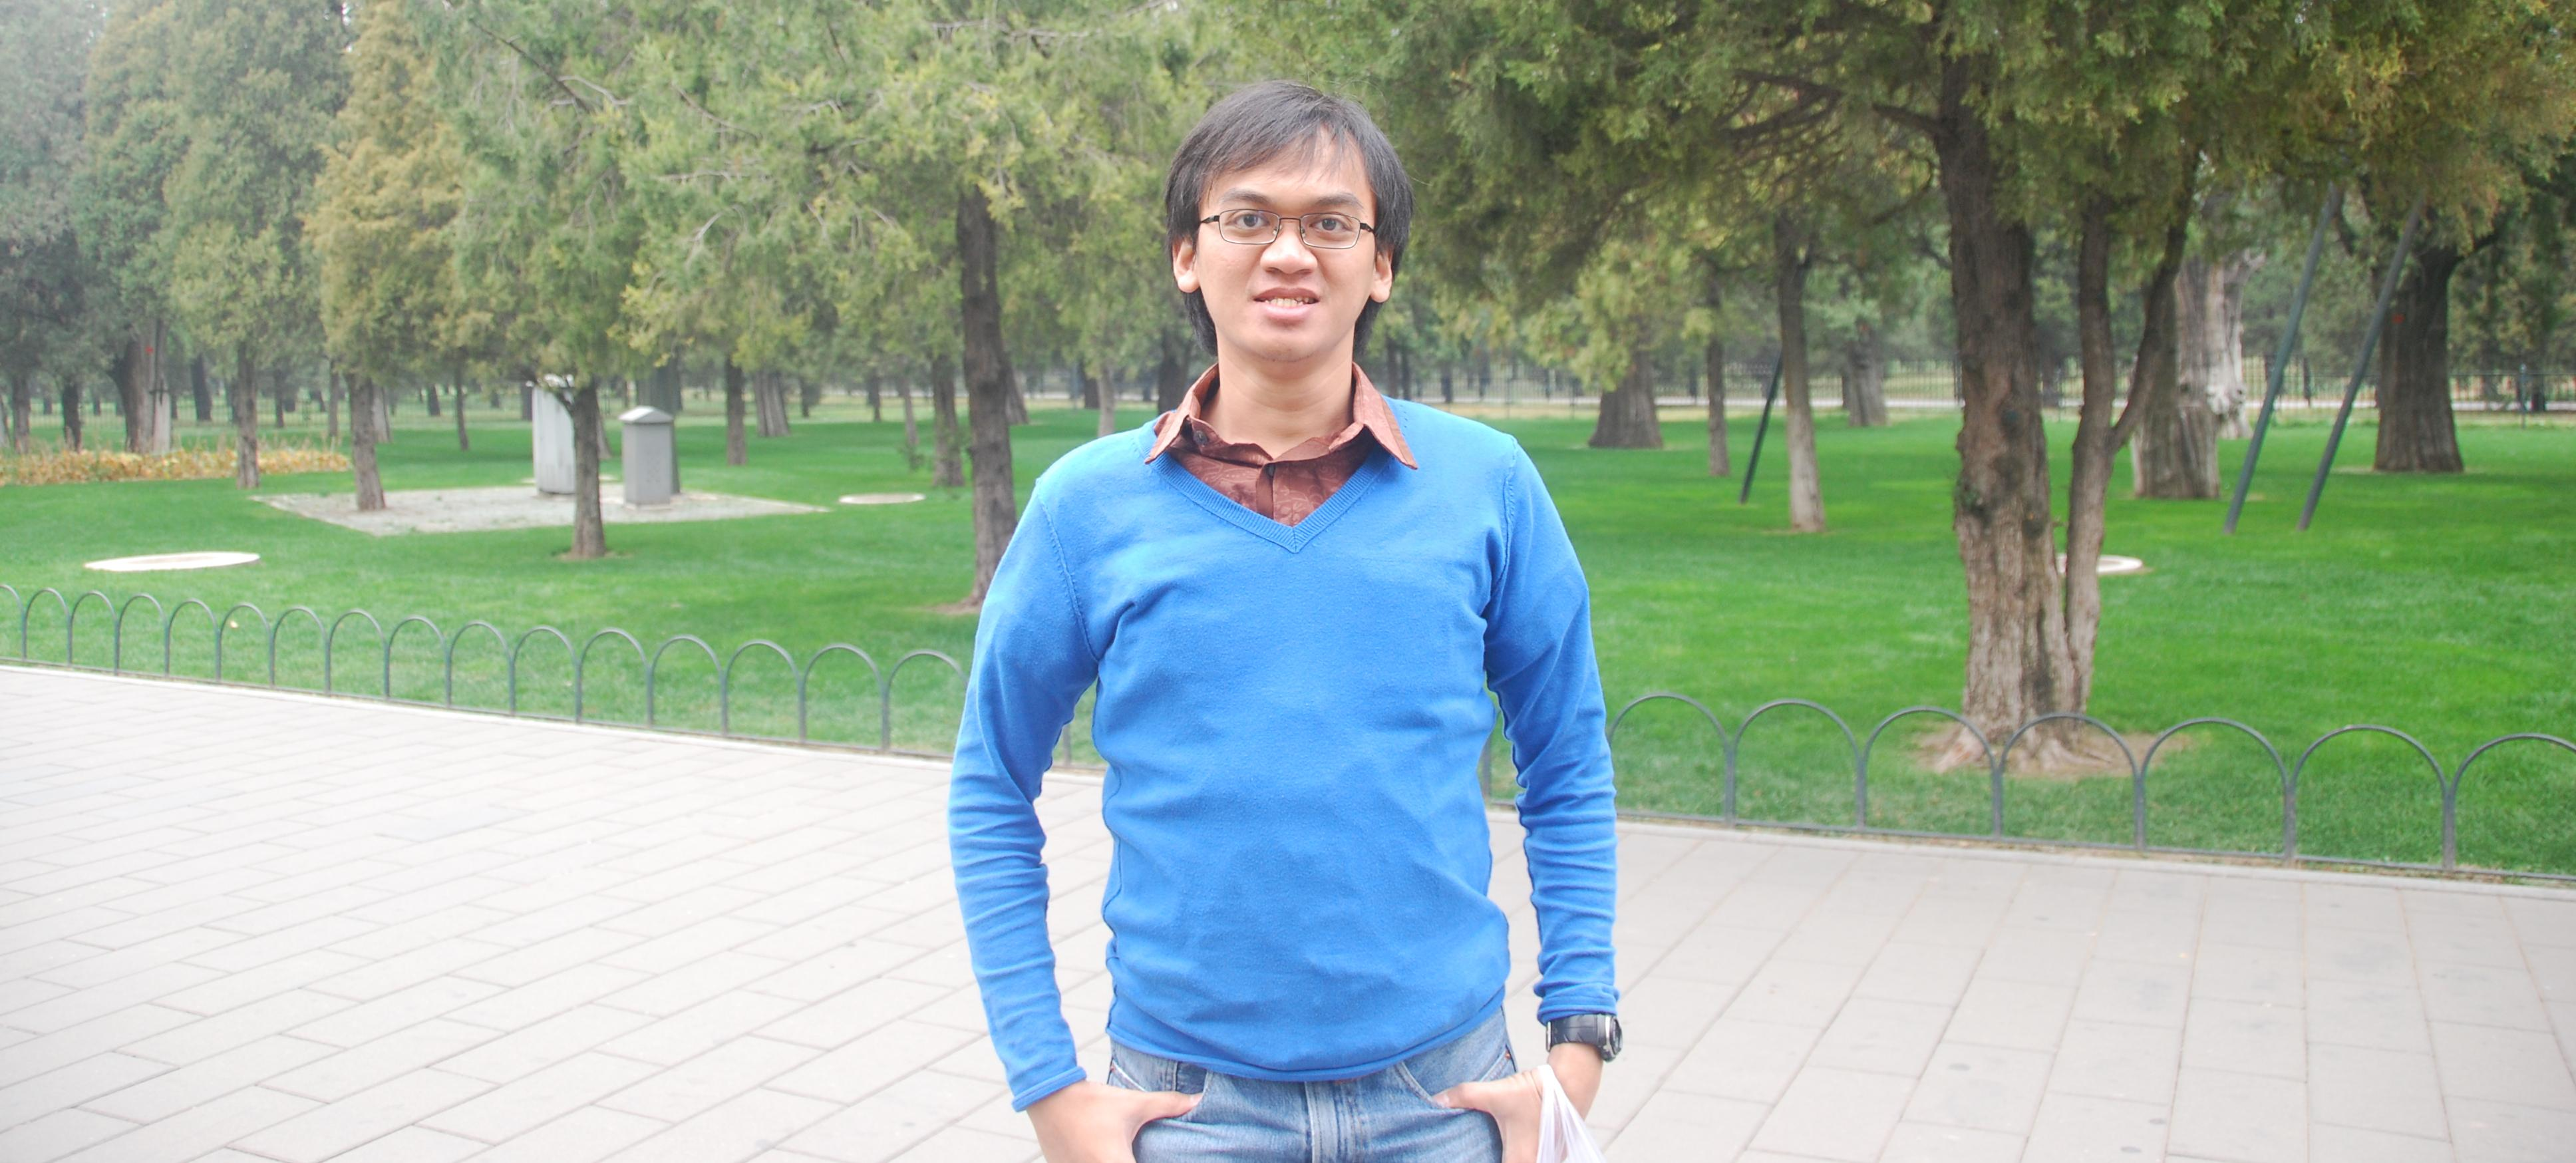
\includegraphics[height=3cm]{za-beijing.jpeg}
			\end{flushleft}
\end{frame}

\section{Mengapa Perlu Secure Coding}

\begin{frame}
	\frametitle{Mengapa Perlu \textit{Secure Coding?}}
	\vskip-1cm
	\begin{columns}		
		\column{0.4\textwidth}
        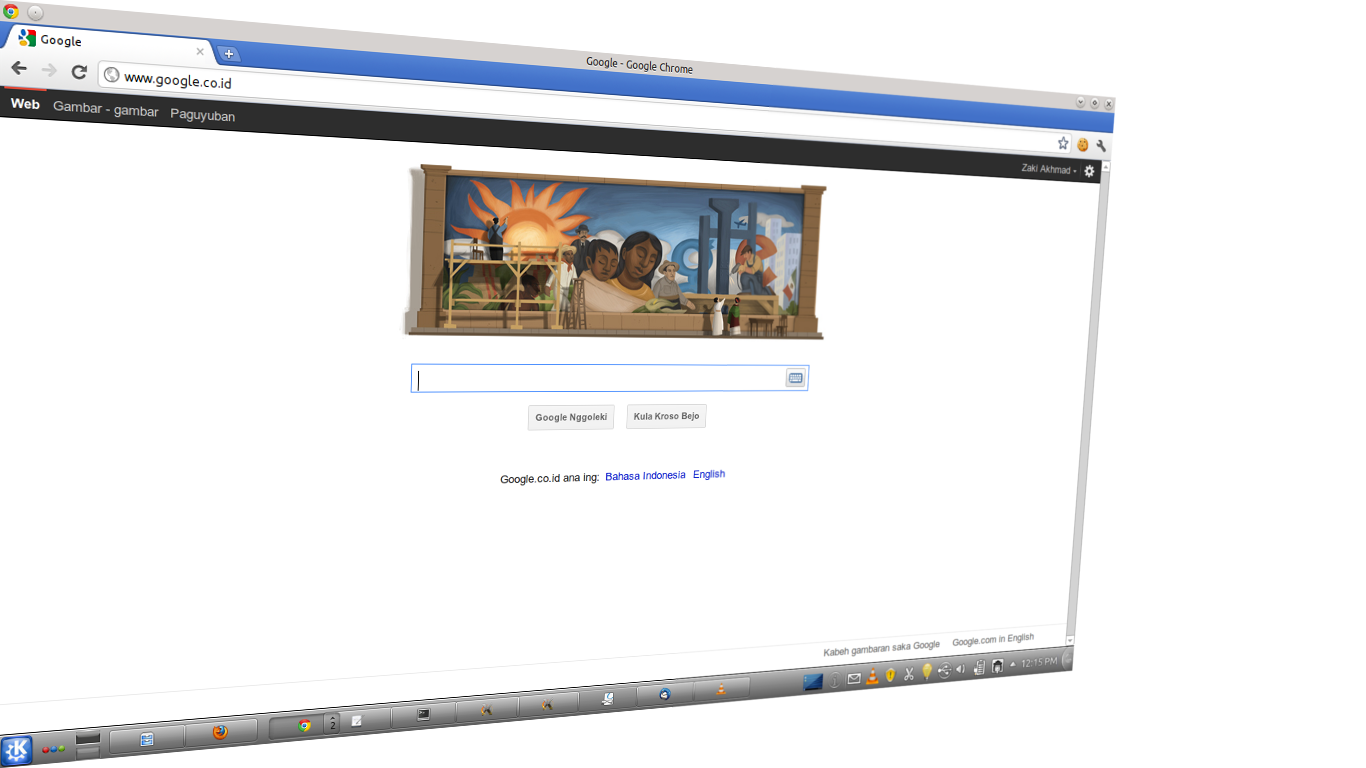
\includegraphics[height=4cm]{google-perspective.png} \pause
        \column{0.6\textwidth}
		\vskip4cm 
		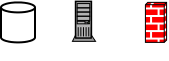
\includegraphics[height=2cm]{network.png} \pause		
	\end{columns}
	\vskip.5cm
	.. . pada praktiknya firewall, IDS/IPS tidak mampu mencegah serangan \textit{SQL injection}. Aplikasi sendiri harus aman. 
\end{frame}

\section{OWASP}

\begin{frame}
	\frametitle{OWASP}
	\begin{columns}
		\column{.4\textwidth}
			\begin{itemize}
				\item Projects
				\begin{itemize}
					\item Tools
					\item Documentations
				\end{itemize}
				\item Conferences
				\item Chapters
			\end{itemize}
		\column{.6\textwidth}
	\begin{center}

\includegraphics[scale=.75]{owasp_3Wx300dpi.jpg}	
\end{center}	
	\end{columns}
\end{frame}

\subsection{Tools}
\begin{frame}
	\frametitle{OWASP}
	\begin{columns}
		\column{.6\textwidth}
			\begin{itemize}
				\item OWASP Tools
				\begin{itemize}
					\item ZAP Proxy {\url{http://goo.gl/Y6oWy}}
					\item WebGoat {\url{http://goo.gl/9RN63}}
					\item GoatDroid {\url{http://goo.gl/k7Rt4}}
				\end{itemize}
			\end{itemize}
		\column{.4\textwidth}
			\begin{center}
				
\includegraphics[height=3cm]{owasp_logo.jpg}
			\end{center}
		\end{columns}
\end{frame}


\begin{frame}
	\frametitle{OWASP}
	\begin{columns}
		\column{.7\textwidth}
			\begin{itemize}
				\item OWASP Tools
				\begin{itemize}
					\item<1> \href{https://www.owasp.org/index.php/OWASP_Zed_Attack_Proxy_Project}{ZAP Proxy} 
					\begin{itemize} 
						\item<1> \scriptsize{Web application proxy}
					\end{itemize}
					\item<2> \href{https://www.owasp.org/index.php/Category:OWASP_WebGoat_Project}{WebGoat}
					\begin{itemize}
						\item<2> \scriptsize{Deliberately insecure J2EE web application}
					\end{itemize}
					\item<3> \href{https://www.owasp.org/index.php/Projects/OWASP_GoatDroid_Project}{GoatDroid}
						\begin{itemize}
							\item<3> \scriptsize{A fully functional training environment for exploring Android mobile application security}
						\end{itemize}
				\end{itemize}
			\end{itemize}
		\column{.3\textwidth}
			\begin{center}
				\includegraphics<1>[height=3cm]{beamer-0.jpg}
				\includegraphics<2>[height=3cm]{beamer-1.jpg}
				\includegraphics<3>[height=3cm]{beamer-2.jpg}
			\end{center}
		\end{columns}
\end{frame}


\subsection{Documentation}

\begin{frame}
	\begin{columns}
		\column{.4\textwidth}
			\begin{itemize}
				\item Dokumentasi OWASP
				\begin{itemize}
					\item {\href{https://www.owasp.org/index.php/Category:OWASP_Top_Ten_Project}{OWASP Top 10}}
					\item {\href{https://www.owasp.org/index.php/OWASP_Testing_Project}{OWASP Testing Guide}}
					\item {\href{}{OWASP Development Guide}}
					\item {\href{https://www.owasp.org/index.php/Projects/OWASP_Development_Guide}{OWASP ASVS}}
					\item ...
				\end{itemize}
			\end{itemize}
		\column{.6\textwidth}
			\begin{center}
				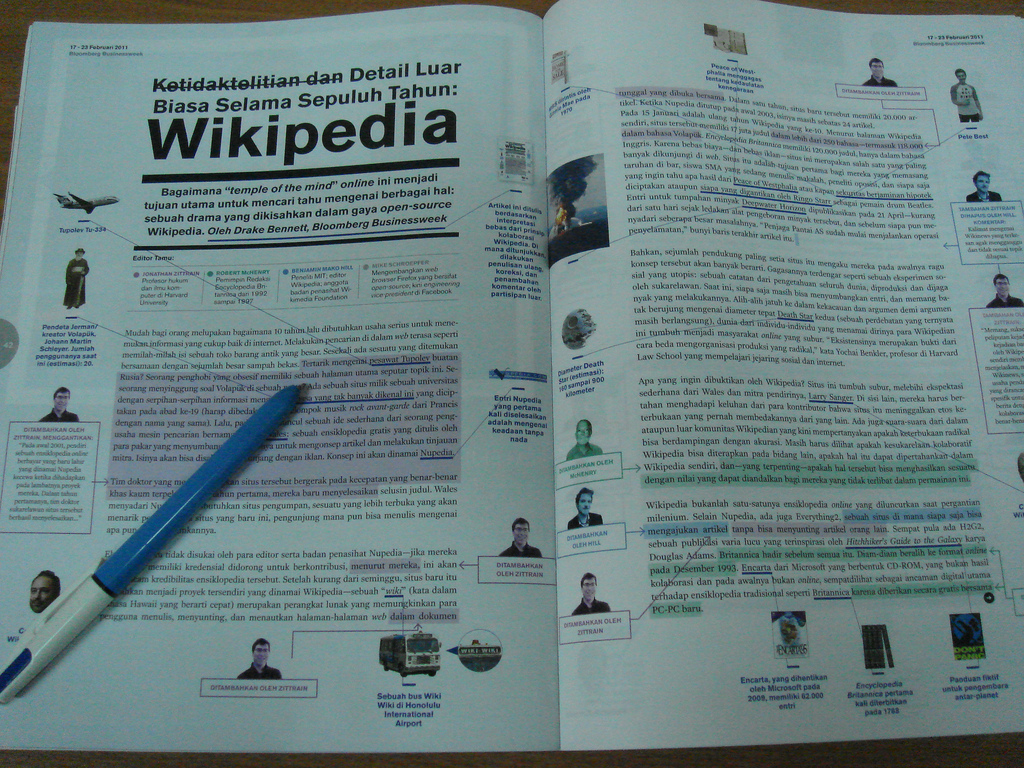
\includegraphics[height=4cm]{wikipedia.jpg}
			\end{center}	
	\end{columns}
\end{frame}

\begin{frame}
	\begin{columns}
		\column{.4\textwidth}
			\begin{itemize}
				\item Dokumentasi OWASP
				\begin{itemize}
				\item<1> OWASP Top 10 
				\item<2> OWASP Testing Guide
				\item<3> OWASP Development Guide
				\item<4> OWASP ASVS
				\end{itemize}
			\end{itemize}		
		\column{.6\textwidth}
			\begin{center}
				\includegraphics<1>[height=5cm]{owasp-top-ten-2010.jpg}
				\includegraphics<2>[height=5cm]{owasp-testing-guide.jpg}
				\includegraphics<3>[height=5cm]{owasp-development-guide.jpg}
				\includegraphics<4>[height=5cm]{owasp-asvs.jpeg}
			\end{center}
	\end{columns}
\end{frame}

\subsection{Conferences} 

\begin{frame}
	\frametitle{Konferensi}
	\begin{center}
		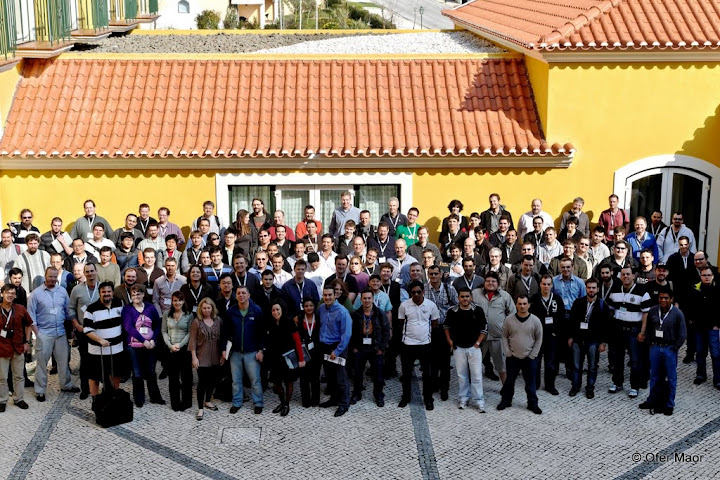
\includegraphics[height=5cm]{owasp-summit.jpg}
		\\ 
		\vskip.5cm
		\small{Summit, Konferensi (Asia-Pasifik, Eropa, Amerika Utara, Amerika Latin)}
	\end{center}	
\end{frame}

\subsection{Chapters}

\begin{frame}
	\frametitle{Chapter}
	\begin{center}
		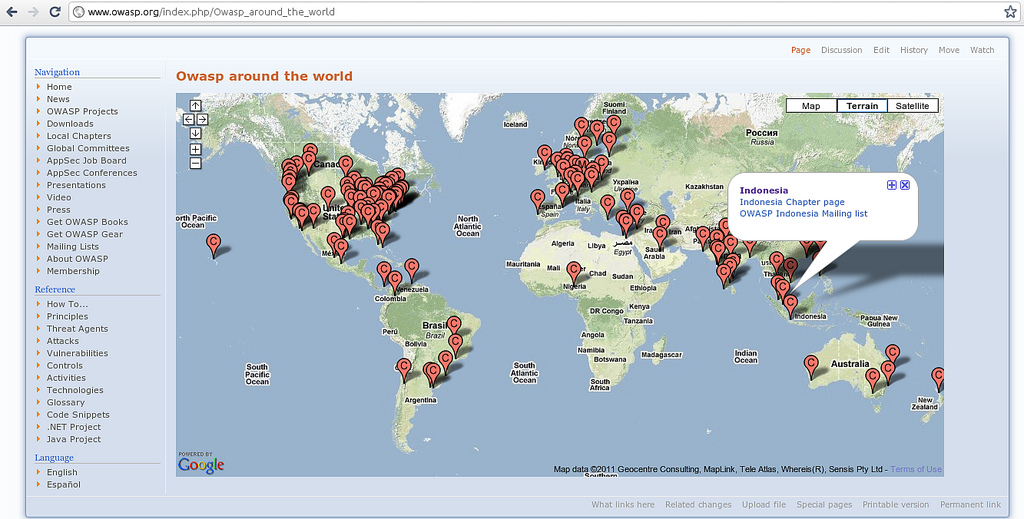
\includegraphics[height=5cm]{owaspid.jpg} 
		\vskip.5cm		
		Singapura, Malaysia, Korea Selatan, \textbf{Indonesia}, Jepang
	\end{center}
\end{frame}

\subsection{OWASP Indonesia}

\begin{frame}
	\frametitle{OWASP Indonesia}
	\begin{center}
		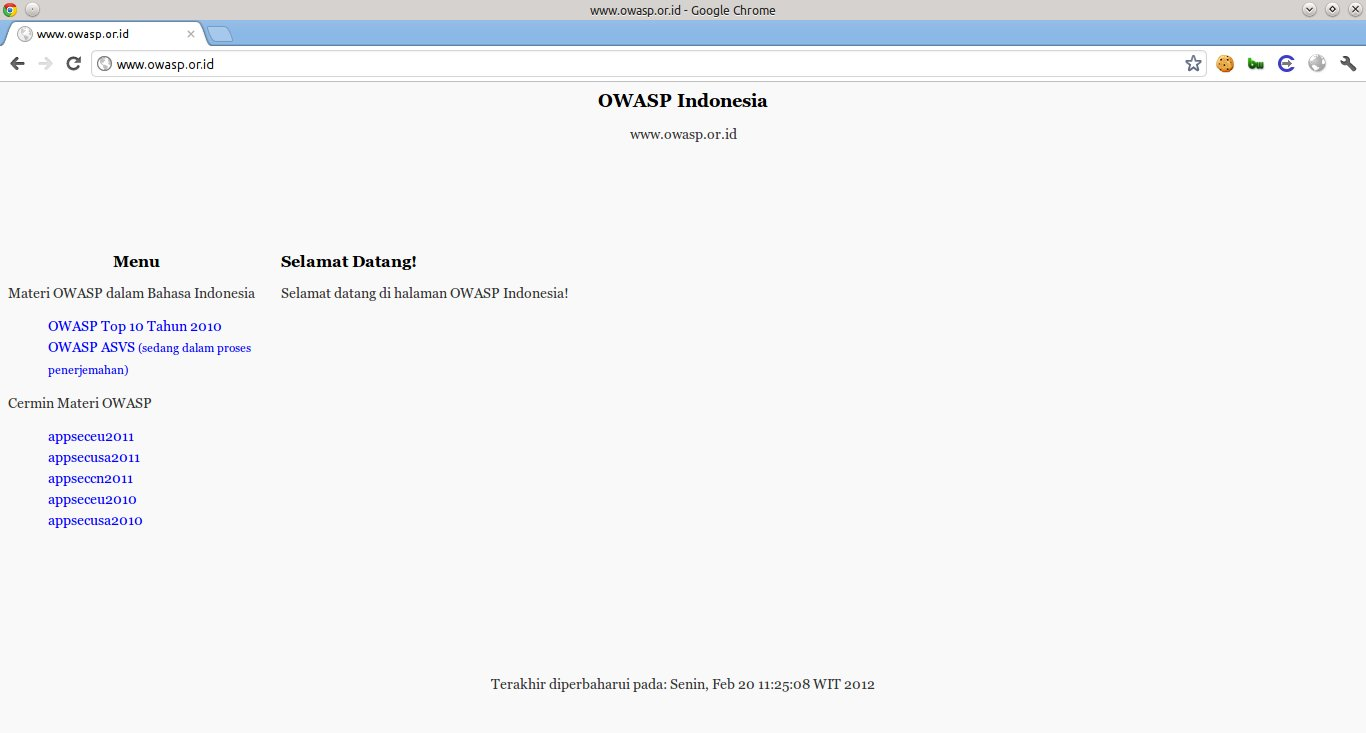
\includegraphics[height=5cm]{owaspid-site.jpg}			
	\end{center}
	\begin{description}
		\item[Situs] {\href{http://www.owasp.or.id}{www.owasp.or.id}}
		\item[Twitter] {\href{http://twitter.com/owaspid}{@owaspid}} \\ 
		\item[Milis] {\href{https://lists.owasp.org/mailman/listinfo/owasp-indonesia}{owasp-indonesia@lists.owasp.org}}
	\end{description}
\end{frame}

\begin{frame}
	\frametitle{OWASP Indonesia}
	\begin{center}	
	\begin{columns}			
		\column{.3\textwidth}
			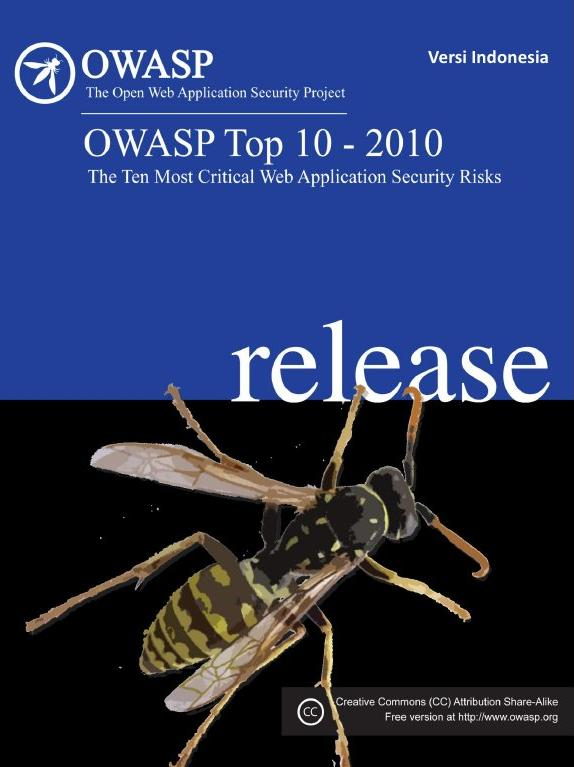
\includegraphics[height=4cm]{owaspid-topten.jpg}
			\\ \begin{center}
					Top 10 - 2010
				\end{center} 		
		\column{.3\textwidth}
			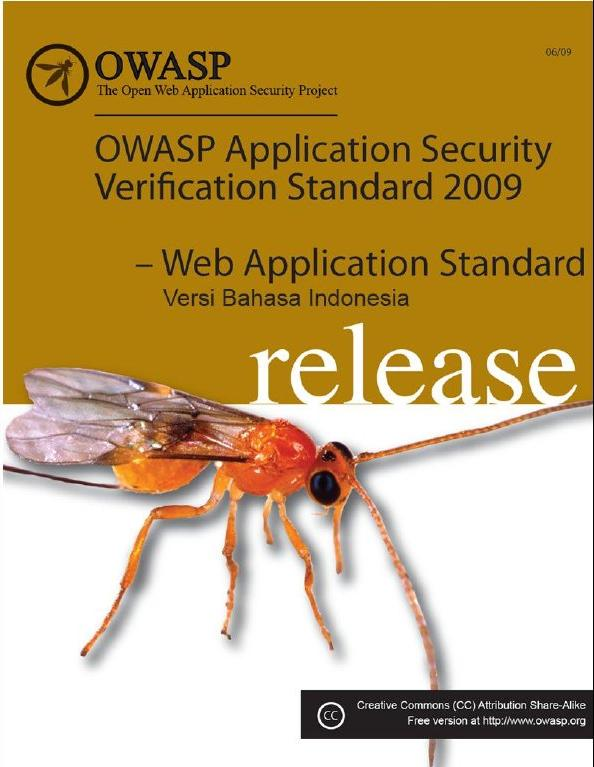
\includegraphics[height=4cm]{owaspid-asvs.jpg}
			\\ \begin{center}
					ASVS
				\end{center}
	\end{columns}
	\vskip1cm Proyek Penerjemahan
	\end{center}
\end{frame}

\subsection{Secure Coding Projects}

\begin{frame}
	\frametitle{\textit{Secure Coding Projects} di OWASP}
	\begin{itemize}
		\item {\href{https://www.owasp.org/index.php/Secure_Coding_Principles}{Secure Coding Principles}}
		\item {\href{https://www.owasp.org/index.php/OWASP_Secure_Coding_Practices_-_Quick_Reference_Guide}{Quick Reference Guide}}
		\item {\href{https://www.owasp.org/index.php/Category:OWASP_Enterprise_Security_API}{ESAPI}}
	\end{itemize}
\end{frame}

\section{Secure Coding}
\subsection{Where is Secure Coding?}

\begin{frame}
	\frametitle{\textbf{Where} is Secure Coding}
	\begin{center}
	%\begin{columns}
	%	\column{.5\textwidth}
	%	\column{.5\textwidth}
			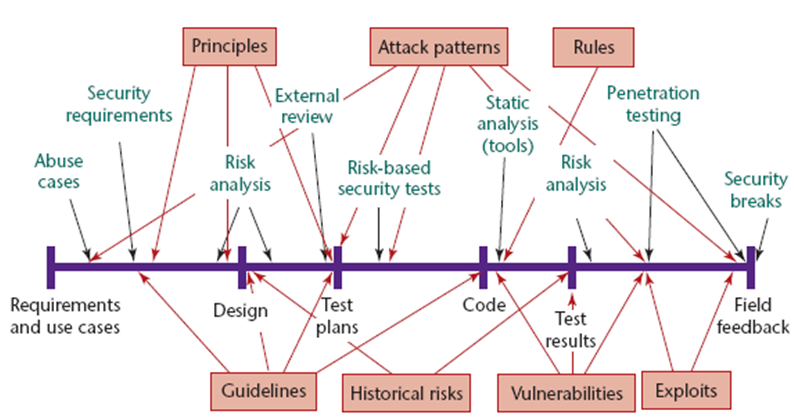
\includegraphics[height=5cm]{securitythroughlifecycle.jpg}
			\\
			\vskip.5cm
			\small{{\href{http://www.amazon.com/Software-Security-Building-In/dp/0321356705}{Software Security, Gary McGraw}}}
	%\end{columns}
	\end{center}
\end{frame}

\subsection{Some Code Snippets}

\begin{frame}[fragile]
	\frametitle{Code Snippets}
			\lstinputlisting{/home/za/Dokumen/csirt/git/sqli-low.php}
	\begin{center}
	Perhatikan baris ke-5 s/d 8
	\end{center}
\end{frame}

\begin{frame}[fragile]
	\frametitle{Code Snippets}
			\lstinputlisting{/home/za/Dokumen/csirt/git/login.php}
	\begin{center}
		Perhatikan baris ke-17
	\end{center}
\end{frame}

\subsection{OWASP Secure Coding - Quick Reference Guide}

\begin{frame}
	\frametitle{OWASP Secure Coding - Quick Reference Guide}
	\underline{Overview}
	\begin{itemize}
		\item Technology agnostic coding practices \pause
		\item What to do, \textbf{not} how to do it \pause
		\item Compact, but comprehensive checklist format \pause
		\item Focuses on secure coding requirements, rather than on vulnerabilities and exploits \pause
		\item Includes a cross-referenced glossary to get \textbf{developers and security folks} talking the same language
	\end{itemize}
\end{frame}

\begin{frame}
	\frametitle{OWASP Secure Coding - Quick Reference Guide}
	\underline{Daftar Isi}
	\begin{enumerate}
		\item Introduction
		\item Software Security Principles Overview
		\item Secure Coding Practices Checklist
		\item Links to Useful Resources
		\item Glossary of Important Terminology
	\end{enumerate}
\end{frame}

\begin{frame}
	\frametitle{OWASP Secure Coding- Quick Reference Guide}
	\underline{Penggunaan}
	\begin{enumerate}
		\item Sebagai dokumen panduan dalam pengembangan
		\item Sebagai dokumen pendukung SDLC
		\item Sebagai dokumen \textit{requirement} dalam \textit{outsource}
		\begin{enumerate}
			\item Identifikasi \textit{security requirement} dalam proyek pengembangan
			\item Masukkan ke dalam RFP dan Kontrak
		\end{enumerate}
	\end{enumerate}
\end{frame}

\begin{frame}
	\frametitle{OWASP Secure Coding - Quick Reference Guide}
	\begin{center}
	\rowcolors{1}{blue!20}{blue!5}
	\begin{tabular}{|c|l|}\hline
		No & Secure Coding Practices Checklist\\
		\hline
		1 & Input Validation \\
		2 & Output Encoding \\
		3 & Authentication and Password Management \\
		4 & Session Management \\
		5 & Access Control \\
		6 & Cryptographic Practices \\ 
		7 & Error Handling and Logging \\
		8 & Data Protection \\
		9 & Communication Security \\
		10 & System Configuration \\
		11 & Database Security \\
		12 & File Management \\
		13 & Memory Management \\
		14 & General Coding Practices \\
		\hline
	\end{tabular}
	\end{center}
\end{frame}

\begin{frame}[fragile]
	\frametitle{OWASP Secure Coding - Quick Reference Guide}
	\underline{Input Validation}
	\begin{itemize}
		\item If any potentially hazardous characters must be allowed as input, be sure that you implement additional controls like output encoding, secure task specific APIs and accounting for the utilization of that data throughout the application. Examples of common hazardous characters include: 
		\begin{verbatim} 
			< > " ' ( )  & + \ \' \"u
		\end{verbatim}
	\end{itemize}
\end{frame}

\begin{frame}
	\frametitle{OWASP Secure Coding - Quick Reference Guide}
	\underline{Authentication and Password Management} \\
	\begin{itemize}
	\item If your application manages a credential store, it should ensure that only crytograpically strong one-way salted hashes of passwords are stored and that the table/file that stores the password and keys is write-able only by the application. (Do not use the MD5 algorithm if it can be avoided)
	\item Use only HTTP POST request to transmit authentication credentials
	\end{itemize}
\end{frame}

\begin{frame}
	\frametitle{OWASP Secure Coding - Quick Reference Guide}
	\underline{Error Handling and Logging} \\
	\begin{itemize}
	\item Do not disclose sensitive information in error responses, including system details, session identifiers or account information
	\item Use error handlers that do not display debugging or stack trace information
	\item Implement generic error messages and use custom error pages
	\end{itemize}
\end{frame}

\section{Referensi}
\begin{frame}
	\frametitle{Referensi/Bacaan Lanjut}
	\begin{itemize}
		\item {\href{http://www.amazon.com/Software-Security-Building-In/dp/0321356705}{Gary McGraw, Software Security}}						
		\item {\href{https://wiki.mozilla.org/WebAppSec/Secure_Coding_Guidelines}{Mozilla Secure Coding Guidelines}}
		\item {\href{https://www.owasp.org/index.php/OWASP_Secure_Coding_Practices_-_Quick_Reference_Guide}{OWASP Secure Coding Practices, Quick Reference Guide}}		
		\item {\href{http://www.dvwa.co.uk}{Damn Vulnerable Web Application}}
	\end{itemize}
\end{frame}


\begin{frame}
	\frametitle{Terima Kasih}
	\begin{center}
	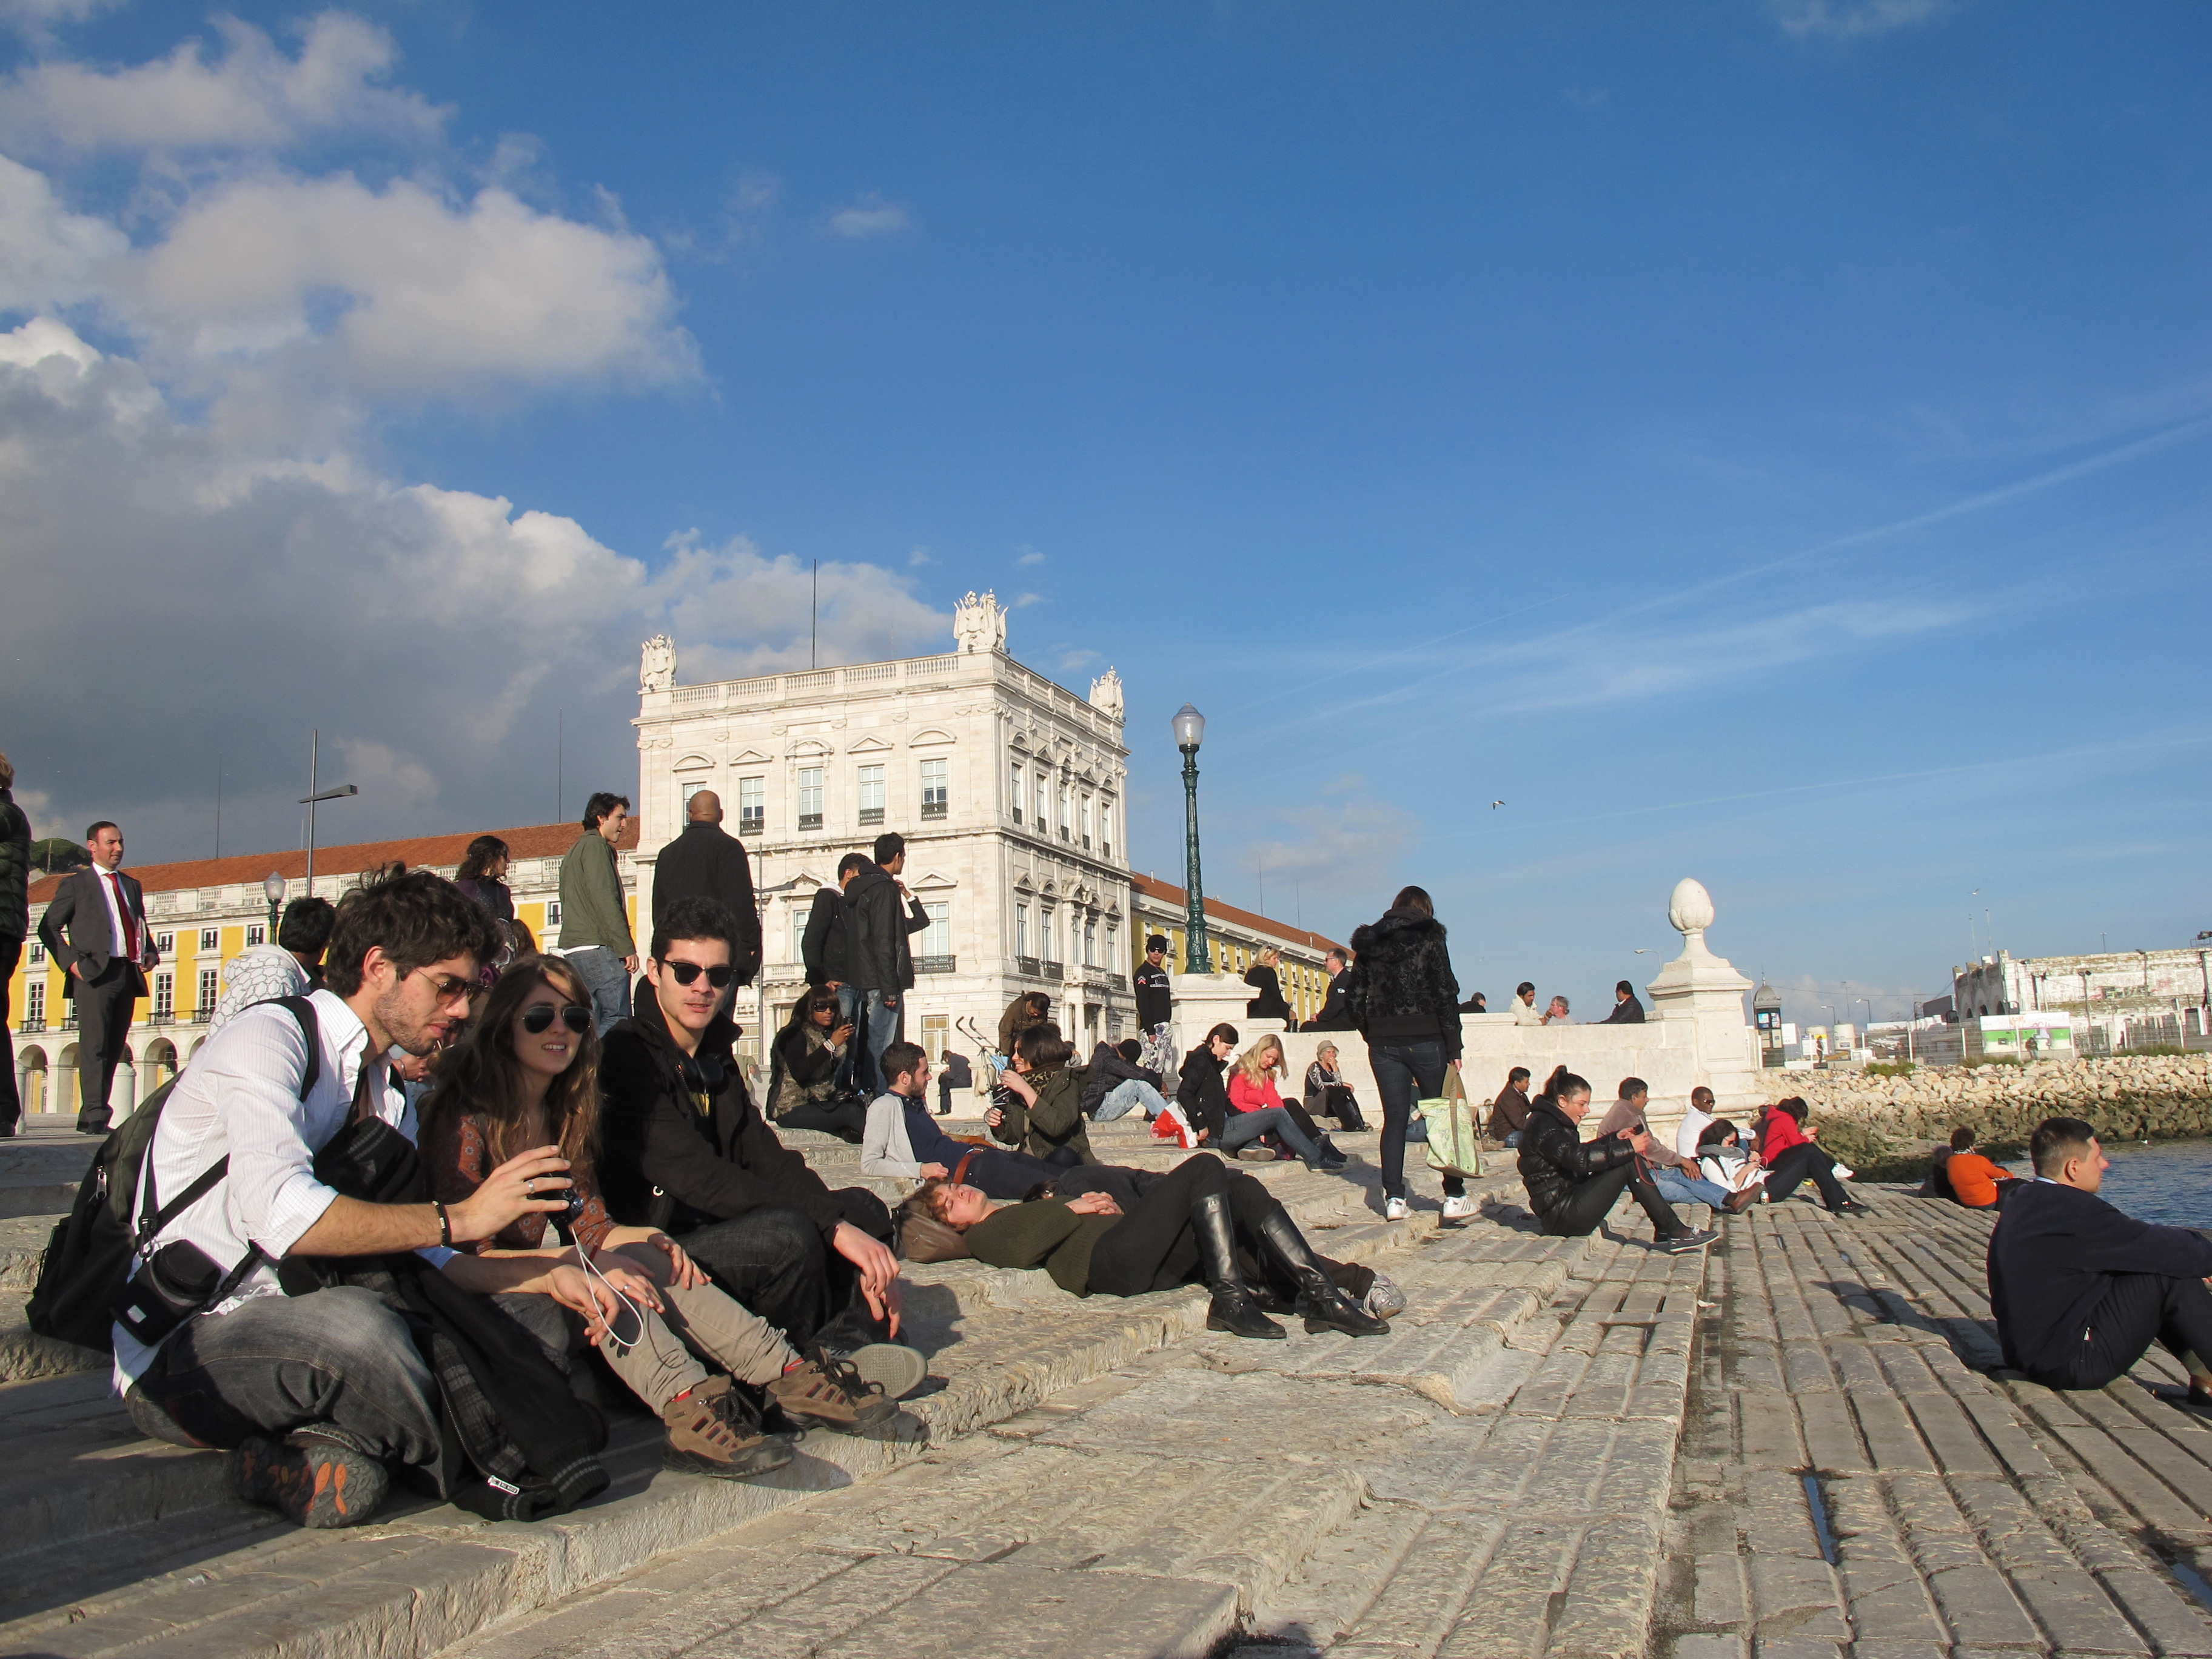
\includegraphics[height=5cm]{IMG_2825.JPG}
		\vskip.5cm \textit{hatur nuhun, matur suwun, \\ thank you, arigatou, danke, merci beaucoup \\}
		\vskip.3cm		
		\tiny{foto-foto {\href{http://flickr.com/zakiakhmad}{flickr.com/zakiakhmad}}}
	\end{center}		
\end{frame}

\end{document}
